\documentclass[a4paper,oneside,12pt]{extreport}

\usepackage{mmap}
\usepackage[T2A]{fontenc}
\usepackage[utf8]{inputenc}
\usepackage[english,russian]{babel}

\usepackage[left=30mm, right=15mm, top=20mm, bottom=20mm]{geometry}

\setlength{\parindent}{1.25cm} % Абзацный отступ

\usepackage{setspace}
\onehalfspacing % Полуторный интервал

\frenchspacing % Равномерные пробелы
\usepackage{indentfirst} % Красная строка

\usepackage{microtype}
\sloppy

\usepackage{titlesec}
\titlespacing*{\chapter}{0pt}{-30pt}{8pt}
\titlespacing*{\section}{\parindent}{*4}{*4}
\titlespacing*{\subsection}{\parindent}{*4}{*4}
\titleformat{\chapter}{\LARGE\bfseries}{\thechapter}{20pt}{\LARGE\bfseries}
\titleformat{\section}{\Large\bfseries}{\thesection}{40pt}{\Large\bfseries}

\usepackage{graphicx}
\usepackage{caption}

\usepackage[unicode,pdftex]{hyperref}
\hypersetup{hidelinks}

\usepackage{amsmath}

%% title begin
\usepackage{wrapfig}

\makeatletter
	\def\vhrulefill#1{\leavevmode\leaders\hrule\@height#1\hfill \kern\z@}
\makeatother
%% title end

%% begin code
\usepackage{listings}
\usepackage{xcolor}

\lstset{
	basicstyle=\footnotesize\ttfamily,
	breakatwhitespace=true,
	breaklines=true,
	commentstyle=\color{gray},
	frame=single,
	keywordstyle=\color{blue},
	stringstyle=\color{red},
	tabsize=8
}

\newcommand{\code}[1]{\texttt{#1}}
%% end code


\begin{document}

\begin{titlepage}
	{\large % 14pt instead of 12pt
	\onehalfspacing
	\centering

	\begin{wrapfigure}[7]{l}{0.14\linewidth}
		\vspace{3mm}
		\hspace{-10mm}
		
\includegraphics[width=0.93\linewidth]{inc/img/bmstu-logo}
	\end{wrapfigure}
	{\singlespacing \footnotesize \bfseries Министерство науки и высшего образования Российской Федерации\\Федеральное государственное бюджетное образовательное учреждение\\высшего образования\\<<Московский государственный технический университет\\имени Н.~Э.~Баумана\\ (национальный исследовательский университет)>>\\(МГТУ им. Н.~Э.~Баумана)\\}

	\vspace{-2.2mm}
	\vhrulefill{0.9mm}\\
	\vspace{-7.5mm}
	\vhrulefill{0.2mm}\\
	\vspace{2mm}

	{\doublespacing \small \raggedright ФАКУЛЬТЕТ \hspace{37mm} «Информатика и системы управления»\\
	КАФЕДРА \hspace{17mm} «Программное обеспечение ЭВМ и информационные технологии»\\}

	\vspace{30mm}

	\textbf{ОТЧЁТ}\\
	По лабораторной работе № 2\\
	По курсу: «Моделирование»\\
	Тема: «Распределение случайных величин»\\
	Вариант: 6 $\equiv$ 2 (mod 4)\\

	\vspace{40mm}

	\begin{flushleft}
		\begin{tabular}{lr}
			\textbf{Студент:}        & Керимов~А.~Ш. \\
			\textbf{Группа:}         & ИУ7-74Б       \\
			\textbf{Оценка (баллы):} & \hrulefill    \\
			\textbf{Преподаватель:}  & Рудаков~И.~В. \\
		\end{tabular}
	\end{flushleft}

	\vfill

	Москва\\
	\the\year\\}
\end{titlepage}

\setcounter{page}{2}


\tableofcontents

\chapter{Формализация}

\section{Задание}

Необходимо промоделировать систему, состоящую из генератора, очереди ёмкостью $L$ и обслуживающего аппарата.
Сообщения могут повторно становиться в очередь с вероятностью $p_{\text{возвр}}$ после обслуживания.
Генерация сообщений происходит по закону равномерного распределения, обработка — по закону нормального распределения.
Определить оптимальную длину очереди, при которой не будет потерянных сообщений.
Реализовать моделирование системы
\begin{enumerate}
	\item принципом $\Delta t$;
	\item событийным принципом.
\end{enumerate}

\section{Принцип $\Delta t$}

Принцип $\Delta t$ заключается в последовательном анализе состояний всех блоков системы в момент $t + \Delta t$  по заданному состоянию блоков в момент $t$.
При этом новое состояние блоков определяется в соответствии с их алгоритмическим описанием с учётом действующих случайных факторов, задаваемых распределениями вероятности.
В результате этого анализа принимается решение о том, какие общесистемные события должны имитироваться программной моделью на данный момент.

Основной недостаток этого принципа: значительные затраты машинного времени на реализацию моделирования системы.
А при недостаточно малом $\Delta t$ появляется опасность пропуска отдельных событий в системе, что исключает возможность получения адекватных результатов при моделировании.

\section{Событийный принцип}

При использовании событийного принципа состояние всех блоков системы анализируется лишь в момент проявления какого-либо события.
Моменты наступления следующего события определяются минимальным значением из списка будущих событий, представляющих собой совокупность моментов ближайшего изменения состояния каждого из блоков.

Проблема пропуска отдельных событий системы при использовании событийного принцип отсутствует, однако недостаток метода заключается в том, что при большом количестве событий системы список необходимо просматривать постоянно.

\chapter{Результат работы}

\begin{figure}[H]
	\centering
	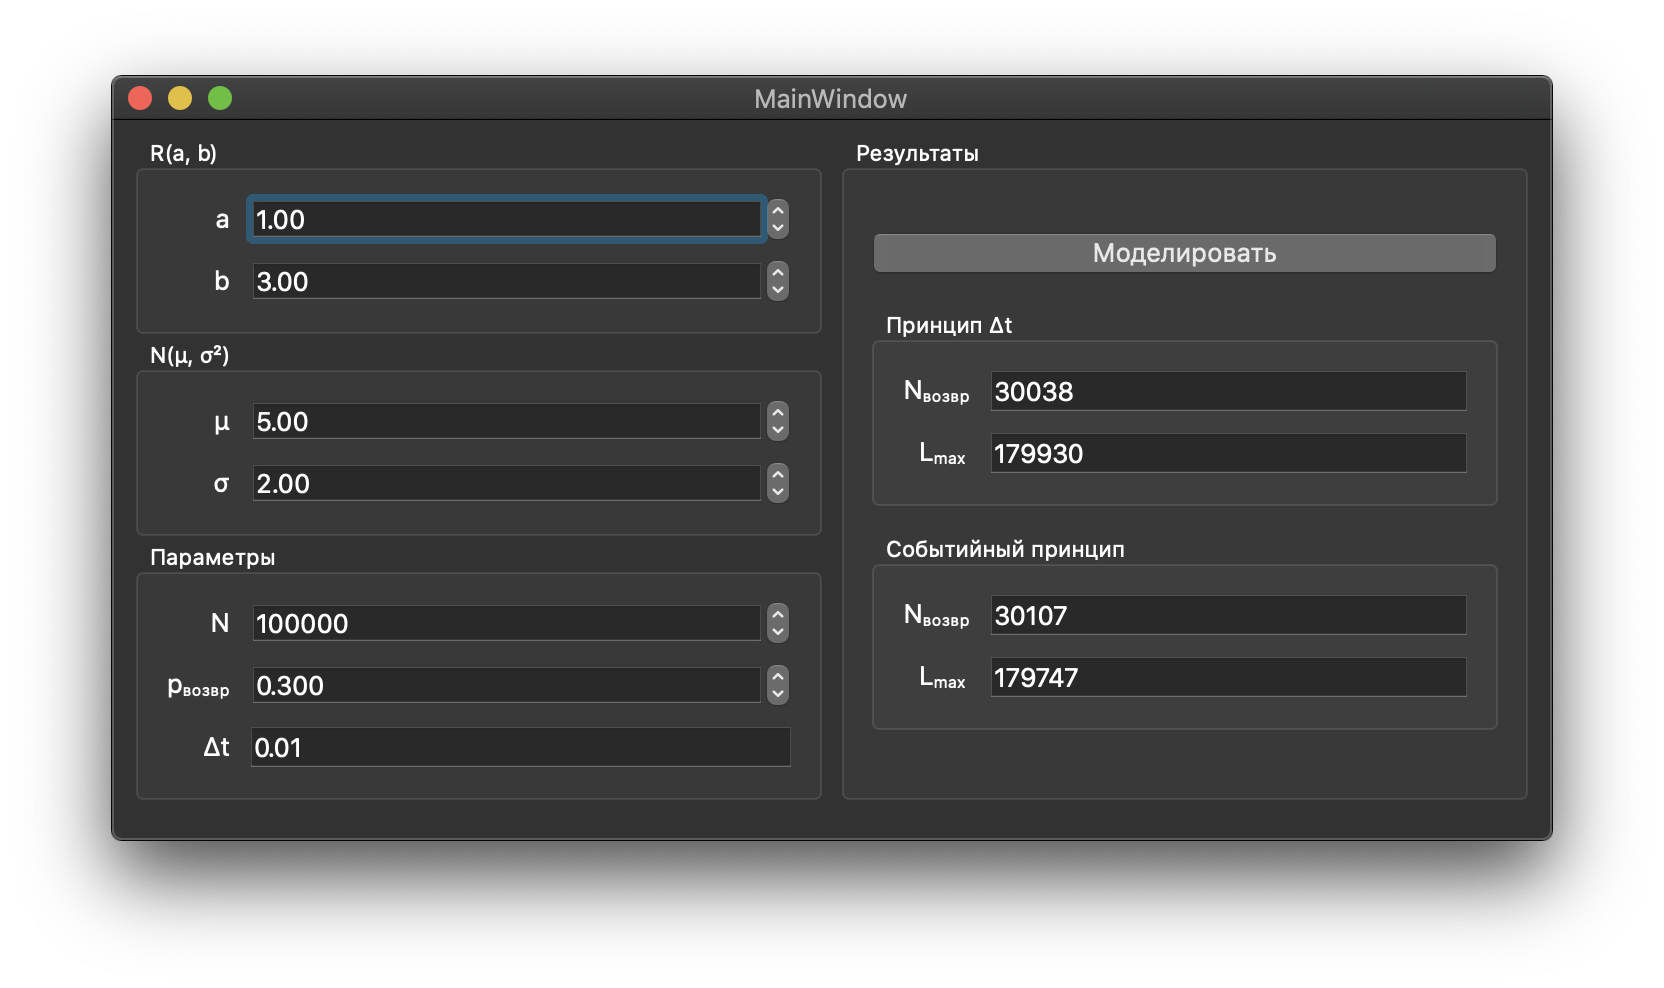
\includegraphics[width=\linewidth]{inc/img/result1.png}
	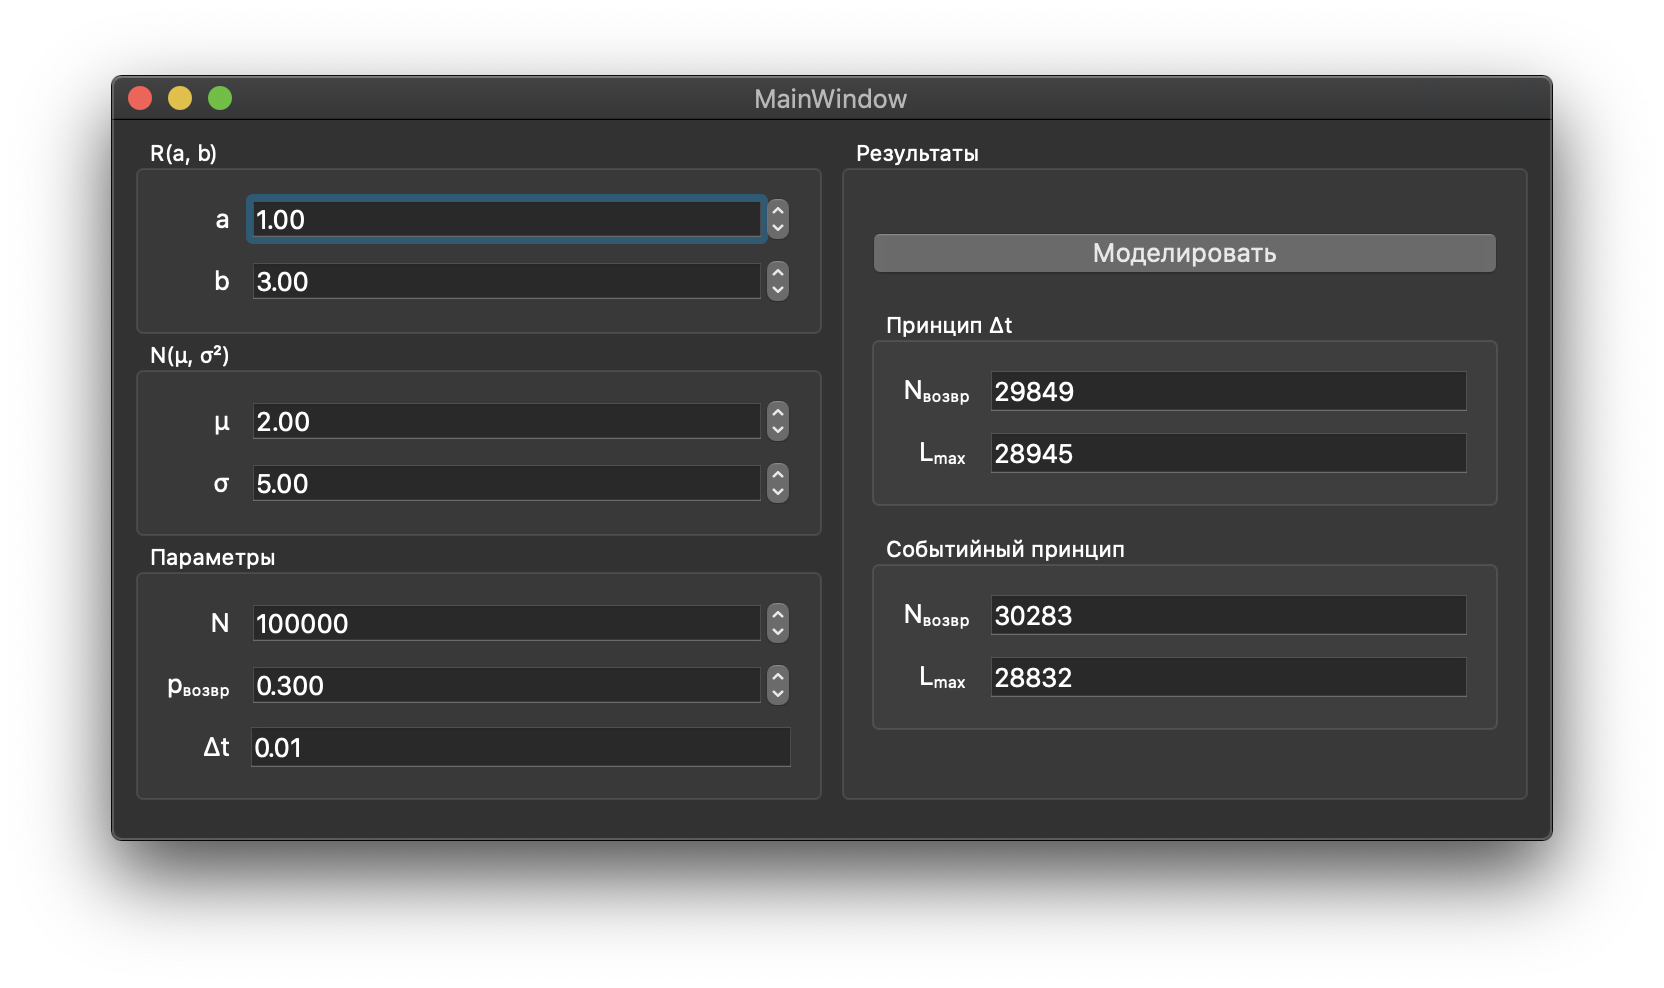
\includegraphics[width=\linewidth]{inc/img/result2.png}
	\caption{Результаты работы программы 1 — 2}
	\label{img:results-12}
\end{figure}

\begin{figure}[H]
	\centering
	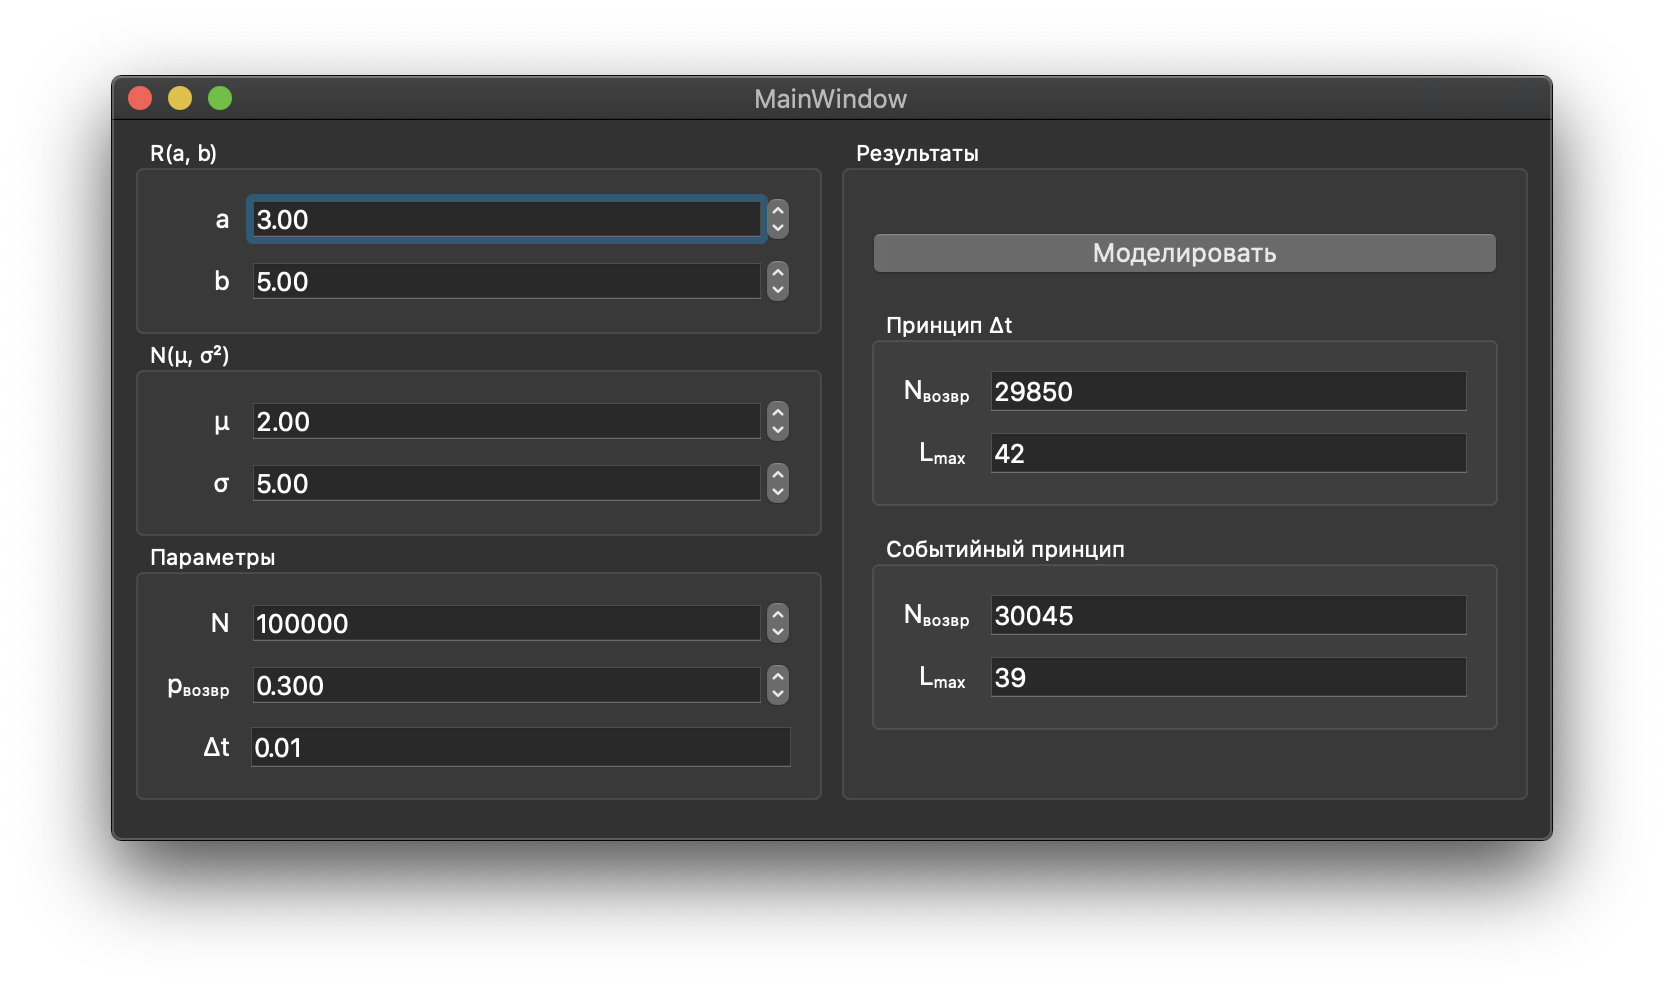
\includegraphics[width=0.8\linewidth]{inc/img/result3.png}
	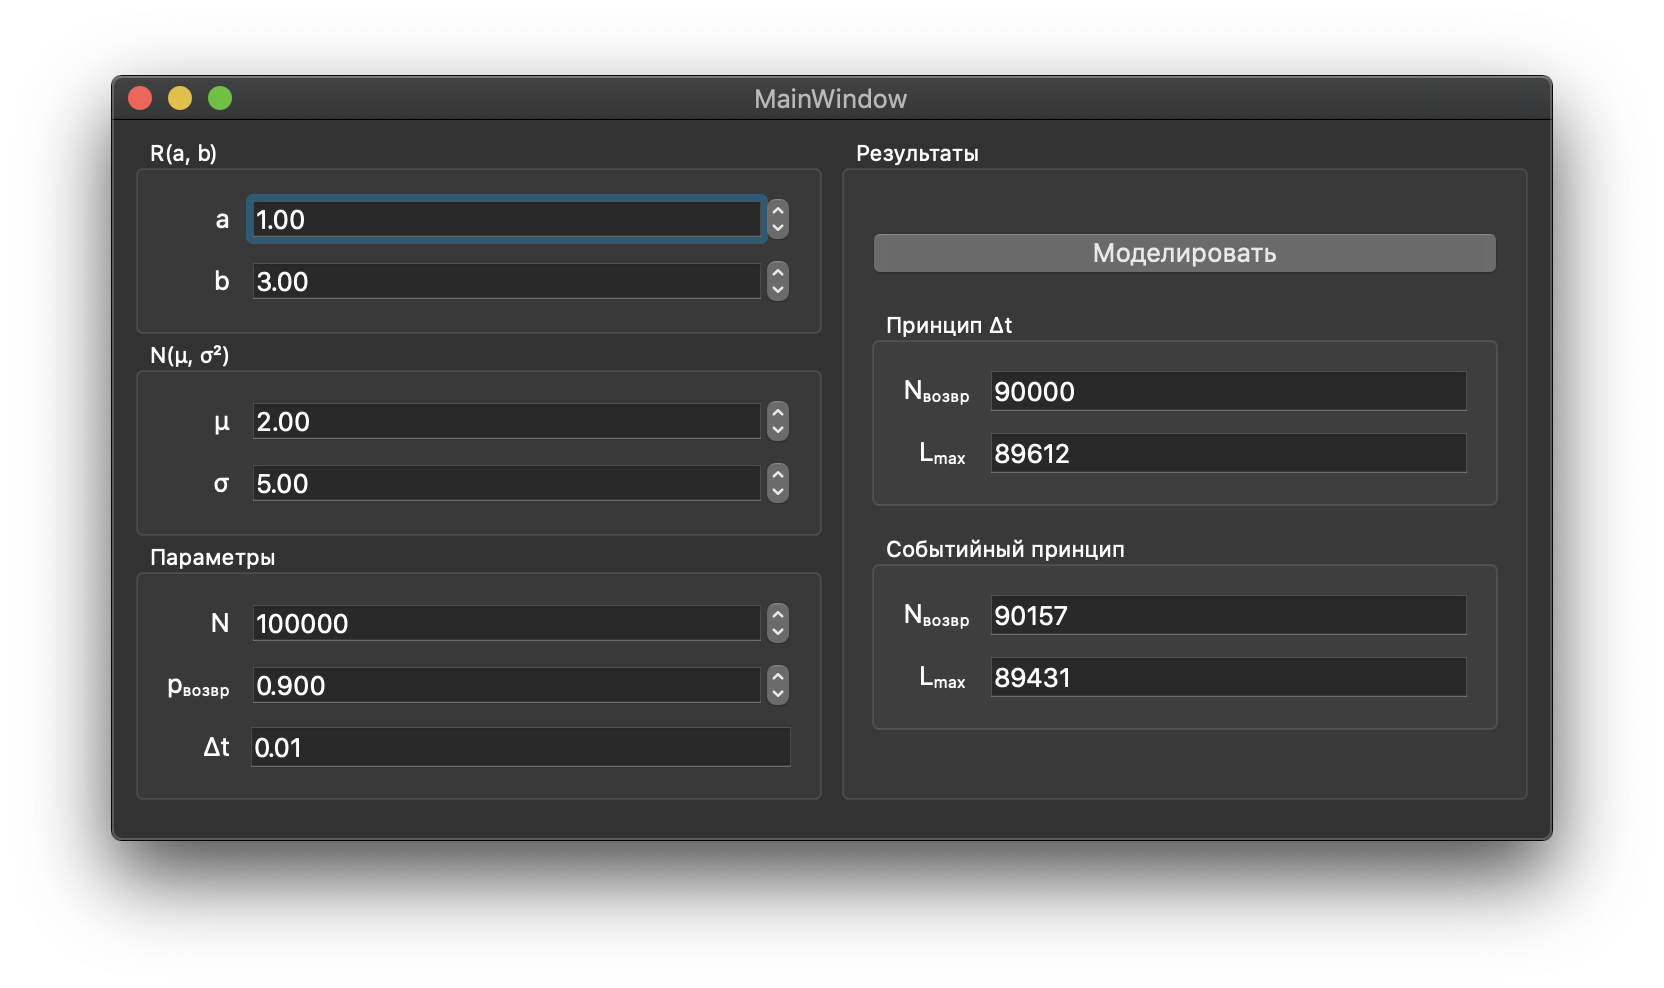
\includegraphics[width=0.8\linewidth]{inc/img/result4.png}
	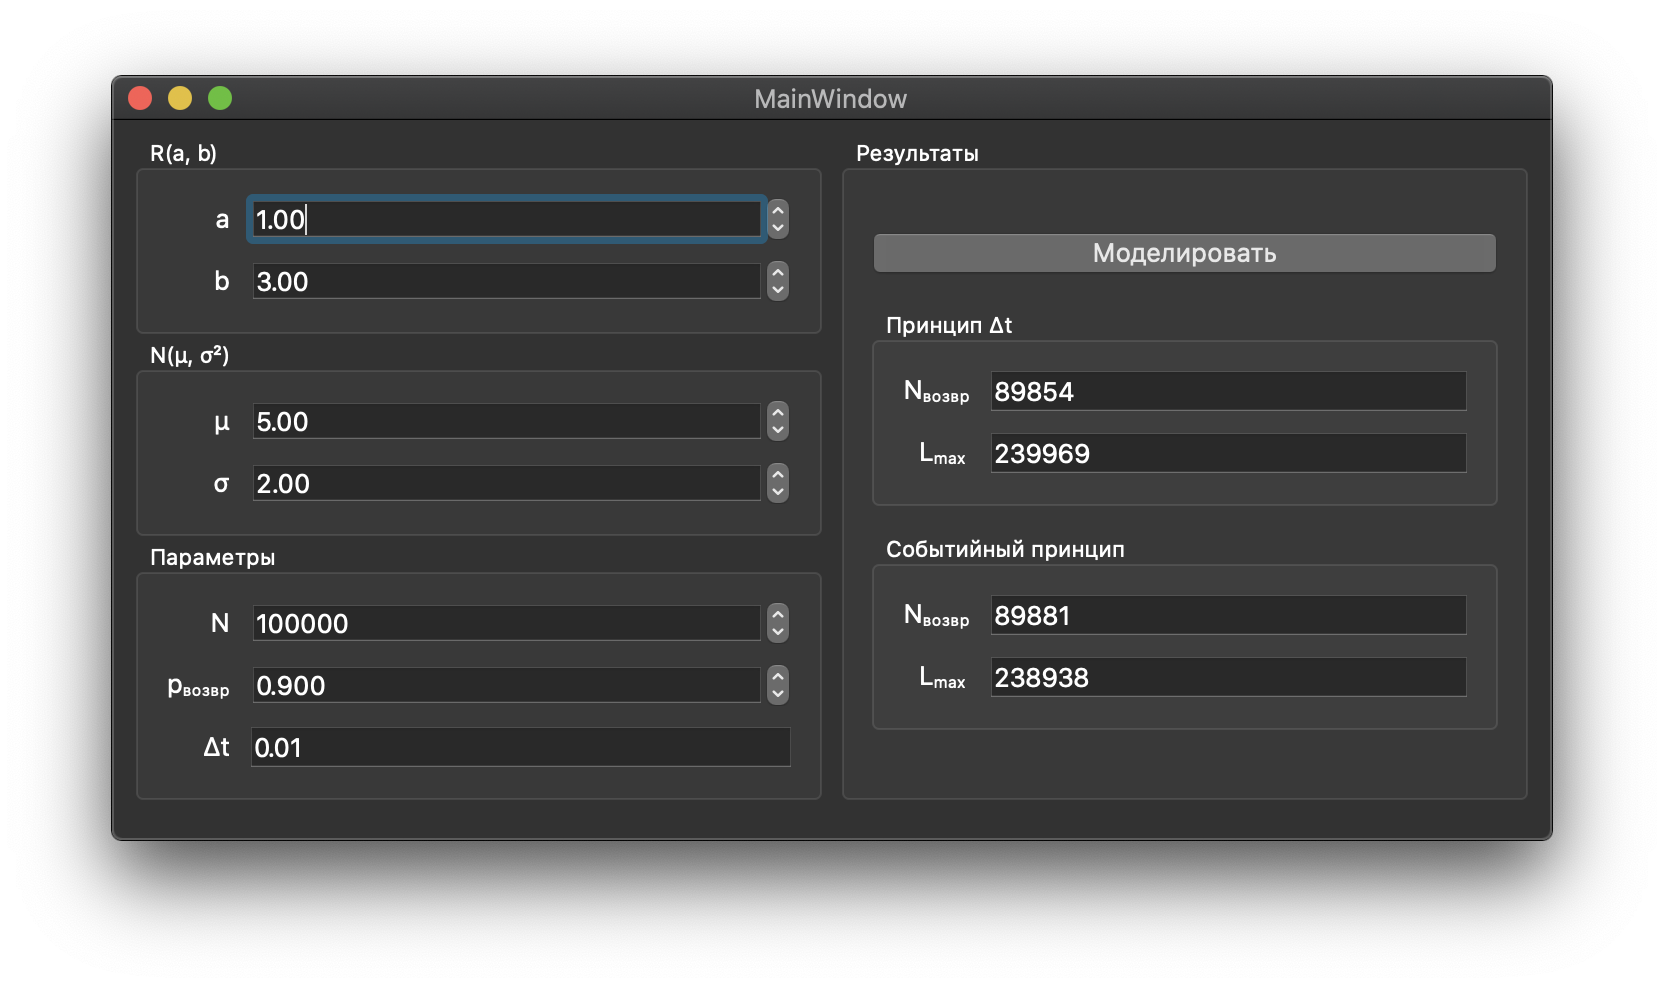
\includegraphics[width=0.8\linewidth]{inc/img/result5.png}
	\caption{Результаты работы программы 3 — 5}
	\label{img:results-35}
\end{figure}

\chapter*{Вывод}
\addcontentsline{toc}{chapter}{Вывод}

Описаны основные принципы имитации управляющей программой алгоритма взаимодействия отдельных устройств в системе — $\Delta t$ и событийный.
Разработана программа, реализующая функционирование СМО с очередью.

Оптимальная длина очереди, при которой не будет потерянных сообщений, равна максимальному количеству сообщений в очереди.

\end{document}
